\section{YAZILIM VE YÖNTEM}

Bu bölümde, Coraza WAF log analizi ve SOM kümeleme sistemi için kullanılan teknolojiler, algoritma detayları ve sistem mimarisi kapsamlı olarak açıklanmaktadır.

\subsection{Sistem Mimarisi ve Teknoloji Yığını}

Geliştirilen sistem, mikroservis mimarisi prensipleri gözetilerek tasarlanmıştır. Sistem altı ana bileşenden oluşmaktadır:

\begin{itemize}
    \item \textbf{Jenkins CI/CD Platform:} Dört farklı pipeline ile otomatik deployment
    \item \textbf{Coraza WAF (Go):} Web uygulama güvenlik duvarı ve JSON log üretimi
    \item \textbf{OWASP ZAP:} Otomatik güvenlik açığı tarama aracı
    \item \textbf{Flask API Servisleri:} Log ve ZAP verilerini sunan REST API'ler
    \item \textbf{Python Analiz Modülü:} SOM algoritması ve gelişmiş veri işleme
    \item \textbf{Streamlit Web Framework:} Kullanıcı etkileşimi ve interaktif görselleştirme
\end{itemize}

\begin{figure}[!ht]
    \centering
    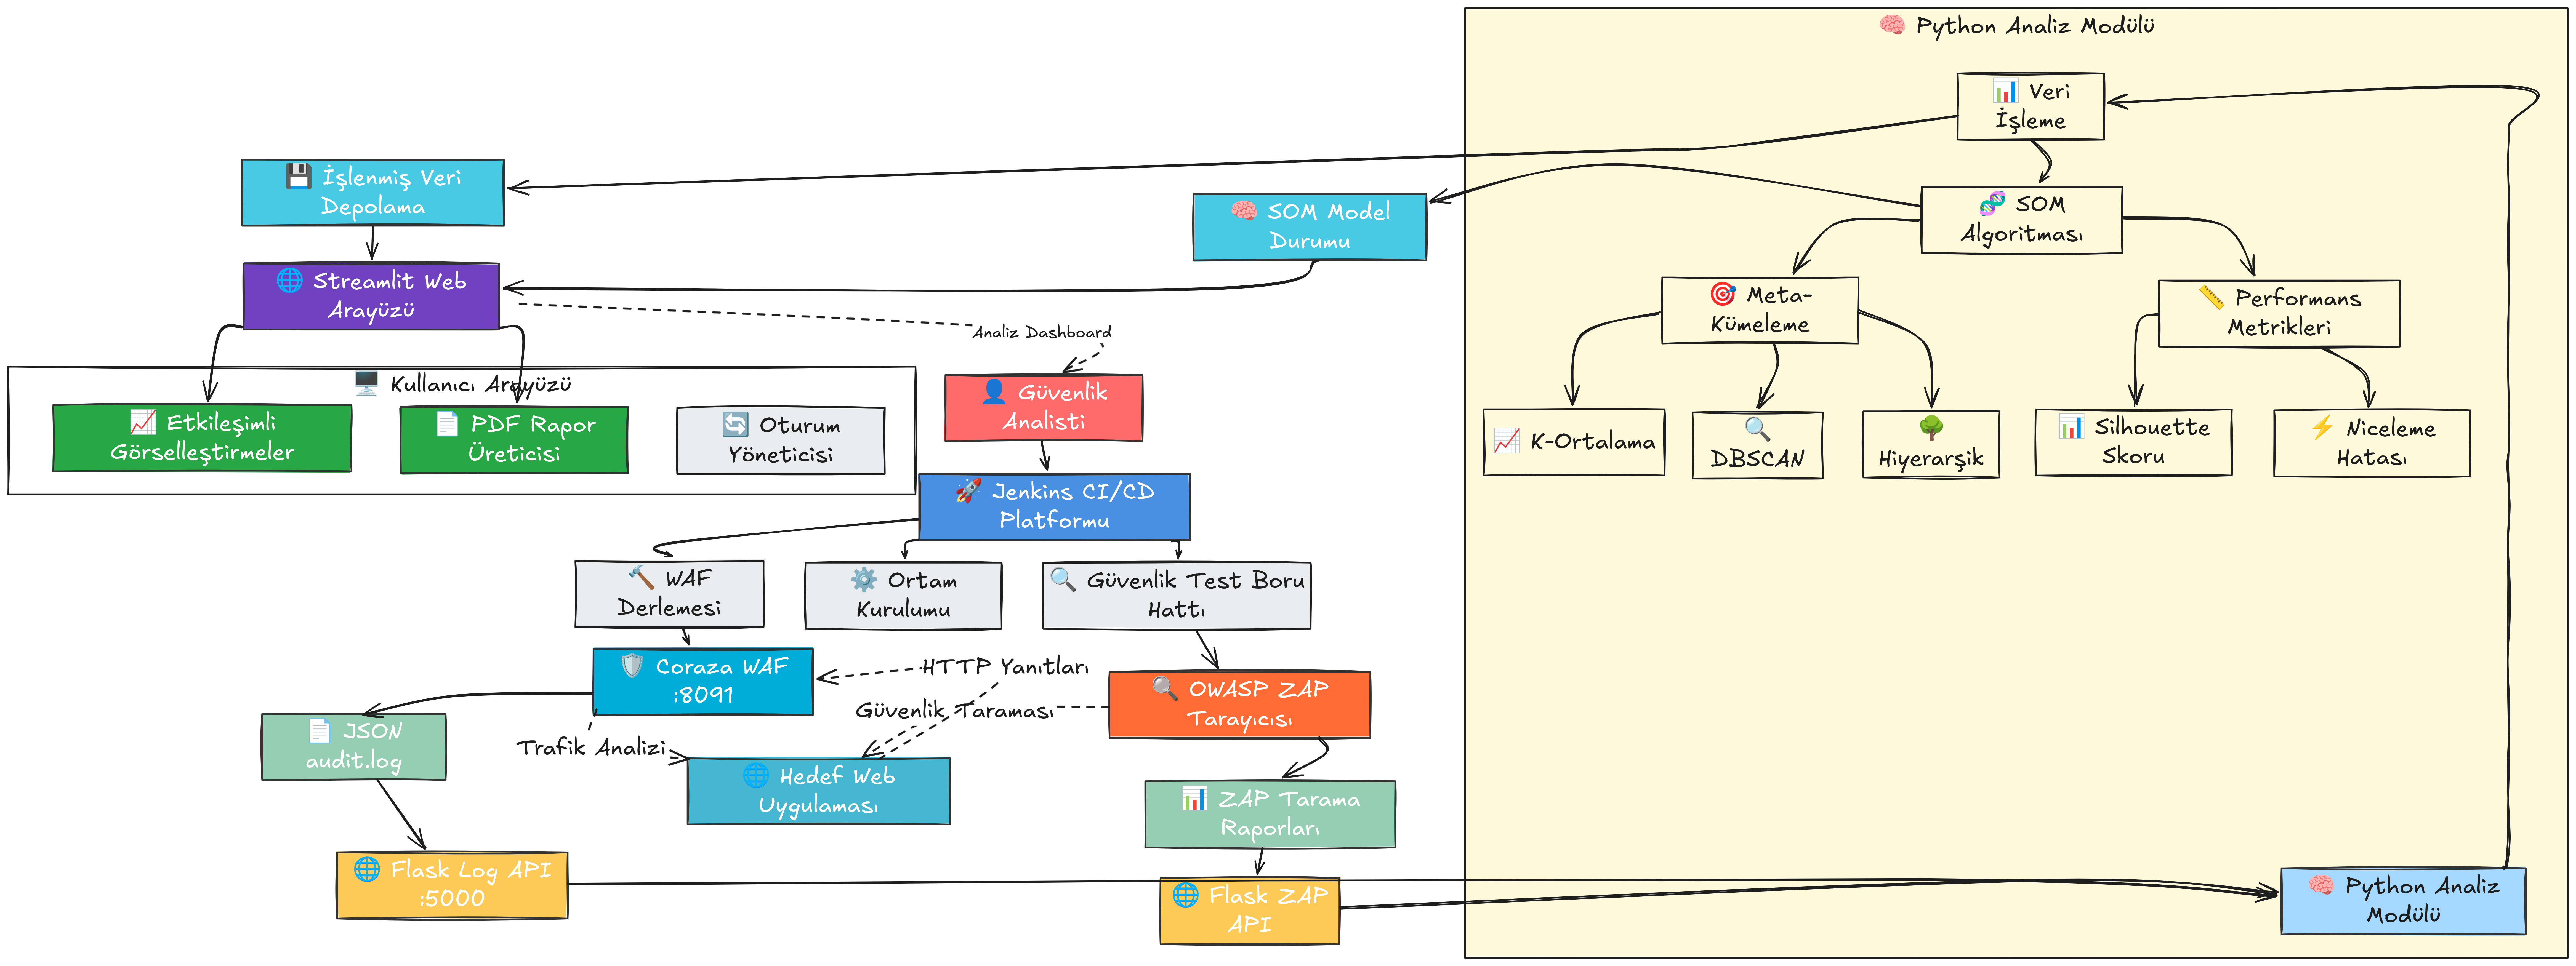
\includegraphics[width=0.95\textwidth]{images/uygulama-mimari-sablonu2.png}
    \caption{Sistem Mimarisi ve Bileşenler Arası Veri Akışı}
    \label{fig:system_architecture}
\end{figure}

Şekil \ref{fig:system_architecture}'de görüldüğü üzere, sistem güvenlik analistinin Jenkins CI/CD platformunu başlatmasıyla çalışmaya başlar. Platform, paralel olarak Coraza WAF derlemesi ve OWASP ZAP güvenlik taramasını gerçekleştirir. Hedef web uygulaması üzerindeki trafik analizi ve güvenlik taraması sonuçları, sırasıyla JSON audit logları ve ZAP raporları olarak üretilir. Bu veriler Flask API servisleri aracılığıyla Python analiz modülüne aktarılır ve SOM algoritması ile meta-kümeleme işlemlerine tabi tutulur. Son olarak, analiz sonuçları Streamlit web arayüzü üzerinden kullanıcıya sunulur.

\newpage

\subsubsection{Teknoloji Yığını Detayları}

Sistem geliştirmesinde kullanılan teknolojiler altı ana kategoride gruplandırılmıştır:

\textbf{1. Arka Uç Teknolojileri:}
\begin{itemize}
    \item \textbf{Go (v1.21):} Coraza WAF gerçekleştirimi ve yüksek başarımlı web servisi
    \item \textbf{Python (v3.8+):} Ana analiz modülü, makine öğrenmesi algoritmaları
    \item \textbf{Flask (v2.3):} REST API servisleri ve mikroservis iletişimi
\end{itemize}

\textbf{2. Makine Öğrenmesi ve Analitik:}
\begin{itemize}
    \item \textbf{MiniSom (v2.3.0):} Kendini Organize Eden Harita gerçekleştirimi \cite{minisom2017}
    \item \textbf{Scikit-learn (v1.3.0):} Üst-kümeleme algoritmaları ve başarım metrikleri
    \item \textbf{NumPy (v1.24):} Sayısal hesaplama ve dizi işlemleri
    \item \textbf{Pandas (v2.0):} Veri manipülasyonu ve JSON işleme
\end{itemize}

\textbf{3. Görselleştirme ve Ön Uç:}
\begin{itemize}
    \item \textbf{Streamlit (v1.28.0):} Etkileşimli web uygulaması çerçevesi \cite{streamlit2023}
    \item \textbf{Plotly (v5.17):} Gelişmiş veri görselleştirme ve etkileşimli grafikler \cite{plotly2015}
    \item \textbf{Matplotlib (v3.7):} İstatistiksel çizim ve grafik üretimi
\end{itemize}

\textbf{4. DevOps ve Otomasyon:}
\begin{itemize}
    \item \textbf{Jenkins (v2.414):} CI/CD boru hattı otomasyonu
    \item \textbf{Docker:} Konteynerleştirme ve dağıtım
    \item \textbf{Groovy:} Boru hattı betik dili
\end{itemize}

\textbf{5. Güvenlik ve Test:}
\begin{itemize}
    \item \textbf{OWASP ZAP (v2.14):} Güvenlik açığı tarama
    \item \textbf{OWASP CRS (v4.0):} WAF için Temel Kural Kümesi
    \item \textbf{Coraza (v3.0):} Modern WAF motoru
\end{itemize}

\newpage

\textbf{6. Veri ve Dokümantasyon:}
\begin{itemize}
    \item \textbf{JSON:} Birincil veri değişim biçimi
    \item \textbf{FPDF (v2.7):} PDF rapor üretimi
    \item \textbf{YAML:} Yapılandırma yönetimi
\end{itemize}

Her teknolojinin projeye katkısı ve seçilme nedenleri aşağıda detaylandırılmıştır.

\subsubsection{Teknolojilerin Projeye Katkıları}

\textbf{MiniSom Kütüphanesi:} Yüksek başarımlı matris işlemleri ve bellek verimli eğitim algoritmaları sağlamaktadır \cite{minisom2017}. Gauss komşuluk fonksiyonu ve dikdörtgen topoloji desteği ile günlük verilerinin topolojik eşleştirme sürecini eniyilemektedir.

\textbf{Streamlit Çerçevesi:} Hızlı prototipleme ve etkileşimli gösterge paneli geliştirme için seçilmiştir \cite{streamlit2023,ozturk2022streamlit}. Oturum durumu yönetimi, gerçek zamanlı veri güncellemeleri ve bileşen tabanlı kullanıcı etkileşimi yetenekleri, güvenlik analistlerinin sistemi etkin kullanmasını sağlamaktadır. Plotly entegrasyonu ile gelişmiş görselleştirme sağlamaktadır \cite{plotly2015}.

\textbf{Flask RESTful API:} Mikroservis mimarisi prensipleri ile günlük verisi sunumu, JSON yanıt biçimlendirmesi ve servisler arası iletişim sağlamaktadır. Jenkins boru hattı entegrasyonu için en uygun başarım sunmaktadır.

\textbf{Jenkins CI/CD Platformu:} Çoklu boru hattı düzenlemesi ve otomatik güvenlik testi için tercih edilmiştir. Groovy betikleme ile dinamik yapılandırma, paralel yürütme ve yapı yönetimi yetenekleri, sürekli güvenlik analizi iş akışını desteklemektedir. Docker konteynerleştirme teknolojisi \cite{kaplan2021docker_guvenlik} ile güvenli ve izole edilmiş çalışma ortamı sağlanmaktadır.

\textbf{Coraza WAF v3:} Go tabanlı modern mimarisi ile tam OWASP CRS uyumluluğu ve kapsamlı güvenlik izleme sağlamaktadır \cite{coraza2023}. Bellek güvenli mimari ve eşzamanlı istek işleme yetenekleri kritik avantajlar sunmaktadır.

\textbf{OWASP ZAP Tarayıcısı:} Kapsamlı saldırı benzetimi ve detaylı raporlama yetenekleri ile güvenlik testi iş akışını tamamlamaktadır \cite{zaproxy2023}.

\newpage

\textbf{Scikit-learn Kütüphanesi:} Üst-kümeleme algoritmaları ve başarım değerlendirme metrikleri için kullanılmıştır \cite{scikit_learn2011}. K-ortalama, DBSCAN, Hiyerarşik kümeleme uygulamaları ile SOM çıktısının sonraki işlemini sağlamaktadır.

\textbf{FPDF Rapor Üreticisi:} Otomatik belgeleme ve denetim izi oluşturma için tercih edilmiştir. Türkçe dil desteği, özel biçimlendirme ve gömülü grafikler ile kapsamlı güvenlik raporları üretmektedir.

\subsection{Self-Organizing Map (SOM) Algoritması}

\textbf{SOM Algoritması Nedir?}

Self-Organizing Map (SOM), yüksek boyutlu verileri düşük boyutlu (genellikle 2D) bir harita üzerinde görselleştiren ve organize eden bir yapay sinir ağı türüdür. SOM'un temel amacı, benzer özelliklere sahip verileri harita üzerinde birbirine yakın konumlarda gruplandırmaktır.

Algoritmanın çalışma prensibi:
\begin{enumerate}
    \item İki boyutlu bir nöron grid'i oluşturulur (örneğin 10x10)
    \item Her nöron, giriş verisi ile aynı boyutta bir ağırlık vektörüne sahiptir
    \item Her eğitim verisi için en benzer nöron (BMU - Best Matching Unit) bulunur
    \item BMU ve komşu nöronların ağırlıkları, giriş verisine daha benzer hale getirilir
    \item Bu işlem tüm veriler için tekrarlanır
    \item Sonuçta, benzer veriler harita üzerinde yakın bölgelerde kümelenir
\end{enumerate}

SOM'un ana avantajları:
- Yüksek boyutlu verileri görselleştirme imkanı
- Küme sayısını önceden belirleme gerektirmez
- Veri yapısını koruyan boyut indirgeme
- Anomali tespiti için kullanılabilir
- İnsan tarafından yorumlanabilir harita üretir

SOM'un dezavantajları:
- Eğitim süreci zaman alabilir
- Grid boyutunun optimize edilmesi gerekir
- Deterministik olmayan sonuçlar (rastgele başlatma nedeniyle)

\newpage

\textbf{BMU (Best Matching Unit) Seçimi:}

\textbf{BMU Nedir?}

Best Matching Unit (BMU), Türkçesi "En İyi Eşleşen Birim", SOM algoritmasının temel kavramlarından biridir. Basitçe, gelen bir veri noktasına en çok benzeyen nöronun bulunması işlemidir.

BMU'nun çalışma mantığı:
\begin{enumerate}
    \item Yeni bir veri noktası geldiğinde, SOM haritasındaki tüm nöronlar incelenir
    \item Her nöronun o veri noktasına olan "mesafesi" hesaplanır
    \item En kısa mesafeye sahip nöron "kazanan" yani BMU olarak seçilir
    \item Bu kazanan nöron ve çevresindeki komşu nöronlar güncellenir
\end{enumerate}

BMU'nun önemi:
- SOM'un öğrenme sürecinin temelini oluşturur
- Benzer verilerin harita üzerinde yakın konumlarda toplanmasını sağlar
- Her veri noktasının hangi bölgeye ait olduğunu belirler
- Anomali tespitinde kritik rol oynar (BMU mesafesi çok büyükse anomali olabilir)

\textbf{Teknik Detaylar:}

Her giriş vektörü $x(t)$ için, en küçük Öklid mesafesine sahip nöron BMU olarak seçilir:

\begin{equation}
c = \arg\min_i ||x(t) - w_i(t)||
\label{eq:bmu_selection}
\end{equation}

\textbf{SOM Güncelleme Formülü:}

\begin{equation}
w_i(t+1) = w_i(t) + \alpha(t) \cdot h_{ci}(t) \cdot [x(t) - w_i(t)]
\label{eq:som_update}
\end{equation}

Burada $\alpha(t)$ öğrenme oranı, $h_{ci}(t)$ komşuluk fonksiyonudur.

\newpage

\textbf{Quantization Error:}

\textbf{Quantization Error Nedir?}

Quantization Error (Niceleme Hatası), SOM'un ne kadar iyi eğitildiğini ölçen temel performans metrikleriuden biridir. Basitçe, her veri noktasının kendi BMU'suna olan uzaklığının ortalamasıdır.

Quantization Error'un anlamı:
\begin{enumerate}
    \item Her veri noktası için en yakın nöron (BMU) bulunur
    \item O veri noktasının BMU'ya olan mesafesi hesaplanır
    \item Tüm veri noktaları için bu mesafelerin ortalaması alınır
    \item Sonuç, SOM'un verilerimizi ne kadar iyi temsil ettiğini gösterir
\end{enumerate}

Quantization Error'un yorumlanması:
- \textbf{Düşük değer:} SOM verileri iyi temsil ediyor, nöronlar verilerine yakın
- \textbf{Yüksek değer:} SOM yetersiz, daha fazla eğitim veya farklı parametreler gerekli
- \textbf{Zaman içindeki azalma:} Eğitim ilerledikçe azalması normal ve istenen durum
- \textbf{Sabit kalma:} Eğitimin durduğunu, konverj olduğunu gösterir

Quantization Error'un kullanım alanları:
- SOM eğitiminin ne zaman duracağına karar vermek
- Farklı grid boyutlarını karşılaştırmak
- Anomali tespiti (anormal yüksek QE değerleri şüpheli)
- Model performansını değerlendirmek

\textbf{Teknik Detaylar:}

\begin{equation}
QE_{avg} = \frac{1}{N} \sum_{i=1}^{N} ||x_i - w_{BMU_i}||
\label{eq:quantization_error}
\end{equation}

\newpage

\subsubsection{Silhouette Score Hesaplama Metodolojisi}

\textbf{Silhouette Score Nedir?}

Silhouette Score, kümeleme algoritmasının ne kadar başarılı olduğunu ölçen bir metriktir. Basitçe, bir veri noktasının kendi kümesindeki diğer noktalara ne kadar yakın olduğunu ve diğer kümelerdeki noktalara ne kadar uzak olduğunu değerlendirir.

Bu metrik şu soruyu cevaplayır: "Bu nokta doğru kümede mi?" 

Silhouette Score'un çalışma prensibi:
\begin{enumerate}
    \item Her veri noktası için kendi kümesindeki diğer noktalara olan ortalama mesafesi hesaplanır (a değeri)
    \item Aynı nokta için, en yakın komşu kümedeki noktalara olan ortalama mesafe hesaplanır (b değeri)
    \item Bu iki değer karşılaştırılarak o noktanın ne kadar "doğru yerde" olduğu belirlenir
    \item Tüm noktalar için bu hesap yapılır ve ortalaması alınır
\end{enumerate}

Silhouette Score'un avantajları:
- -1 ile +1 arasında değer alır, yorumlaması kolaydır
- Küme sayısının optimal olup olmadığını gösterir
- Hem küme içi sıkılığı hem de kümeler arası ayrılığı değerlendirir
- Farklı algoritmaları karşılaştırmak için kullanılabilir

Sonuçların yorumlanması:
- +1'e yakın: Mükemmel kümeleme, noktalar doğru yerde
- 0'a yakın: Belirsiz durum, nokta küme sınırında
- -1'e yakın: Yanlış kümeleme, nokta yanlış yerde

\textbf{Teknik Detaylar:}

Silhouette Score, her bir veri noktasının kendi kümesine ne kadar iyi ait olduğunu ve diğer kümelere ne kadar benzemediğini ölçer. Bir veri noktası $i$ için silhouette katsayısı aşağıdaki formülle hesaplanır:

\begin{equation}
s(i) = \frac{b(i) - a(i)}{\max(a(i), b(i))}
\label{eq:silhouette_score}
\end{equation}

\newpage

Burada:
\begin{itemize}
    \item $a(i)$: Nokta $i$'nin kendi kümesindeki diğer noktalara olan ortalama mesafesi (küme içi mesafe)
    \item $b(i)$: Nokta $i$'nin en yakın komşu kümedeki noktalara olan ortalama mesafesi (kümeler arası mesafe)
\end{itemize}

\textbf{Matematiksel Detaylar:}

\begin{equation}
a(i) = \frac{1}{|C_I| - 1} \sum_{j \in C_I, j \neq i} d(i,j)
\label{eq:intra_cluster_distance}
\end{equation}

\begin{equation}
b(i) = \min_{J \neq I} \frac{1}{|C_J|} \sum_{j \in C_J} d(i,j)
\label{eq:inter_cluster_distance}
\end{equation}

\textbf{Silhouette Score Yorumlama:}
\begin{itemize}
    \item $s(i) \approx 1$: Nokta doğru kümeye atanmış
    \item $s(i) \approx 0$: Nokta küme sınırında 
    \item $s(i) \approx -1$: Nokta yanlış kümeye atanmış
\end{itemize}

Genel Silhouette Score, tüm noktaların silhouette katsayılarının ortalamasıdır:

\begin{equation}
\text{Silhouette Score} = \frac{1}{n} \sum_{i=1}^{n} s(i)
\label{eq:overall_silhouette}
\end{equation}

\newpage

\subsubsection{Sistem Parametreleri}

Sistemde kullanılan SOM parametreleri:

\begin{itemize}
    \item \textbf{Grid Boyutu:} $\sqrt{5 \cdot \sqrt{n}}$ (n: veri sayısı)
    \item \textbf{Sigma:} Grid boyutunun yarısı
    \item \textbf{Öğrenme Oranı:} 0.5 başlangıç değeri
    \item \textbf{İterasyon:} 1000 (kullanıcı ayarlanabilir)
\end{itemize}

\subsection{Veri Önişleme ve Analiz Stratejisi}

\subsubsection{Veri Toplama ve Doğrulama Metodolojisi}

Sistemin veri toplama süreci aşağıdaki katmanlı yapıdan oluşmaktadır:

\begin{enumerate}
    \item \textbf{Kaynak Tanımlama:} Coraza WAF \texttt{audit.log} dosyaları ve ZAP tarama sonuçları
    \item \textbf{Biçim Doğrulama:} JSON şema uyumluluğu ve yapı doğrulaması
    \item \textbf{Kalite Kontrolü:} Eksik alan tespiti, veri türü doğrulaması
    \item \textbf{Veri Temizleme:} Aykırı değer tespiti, gürültü azaltma ve veri standardizasyonu
    \item \textbf{Özellik Mühendisliği:} Alana özgü özellik çıkarımı ve normalleştirme
\end{enumerate}

\begin{figure}[!ht]
    \centering
    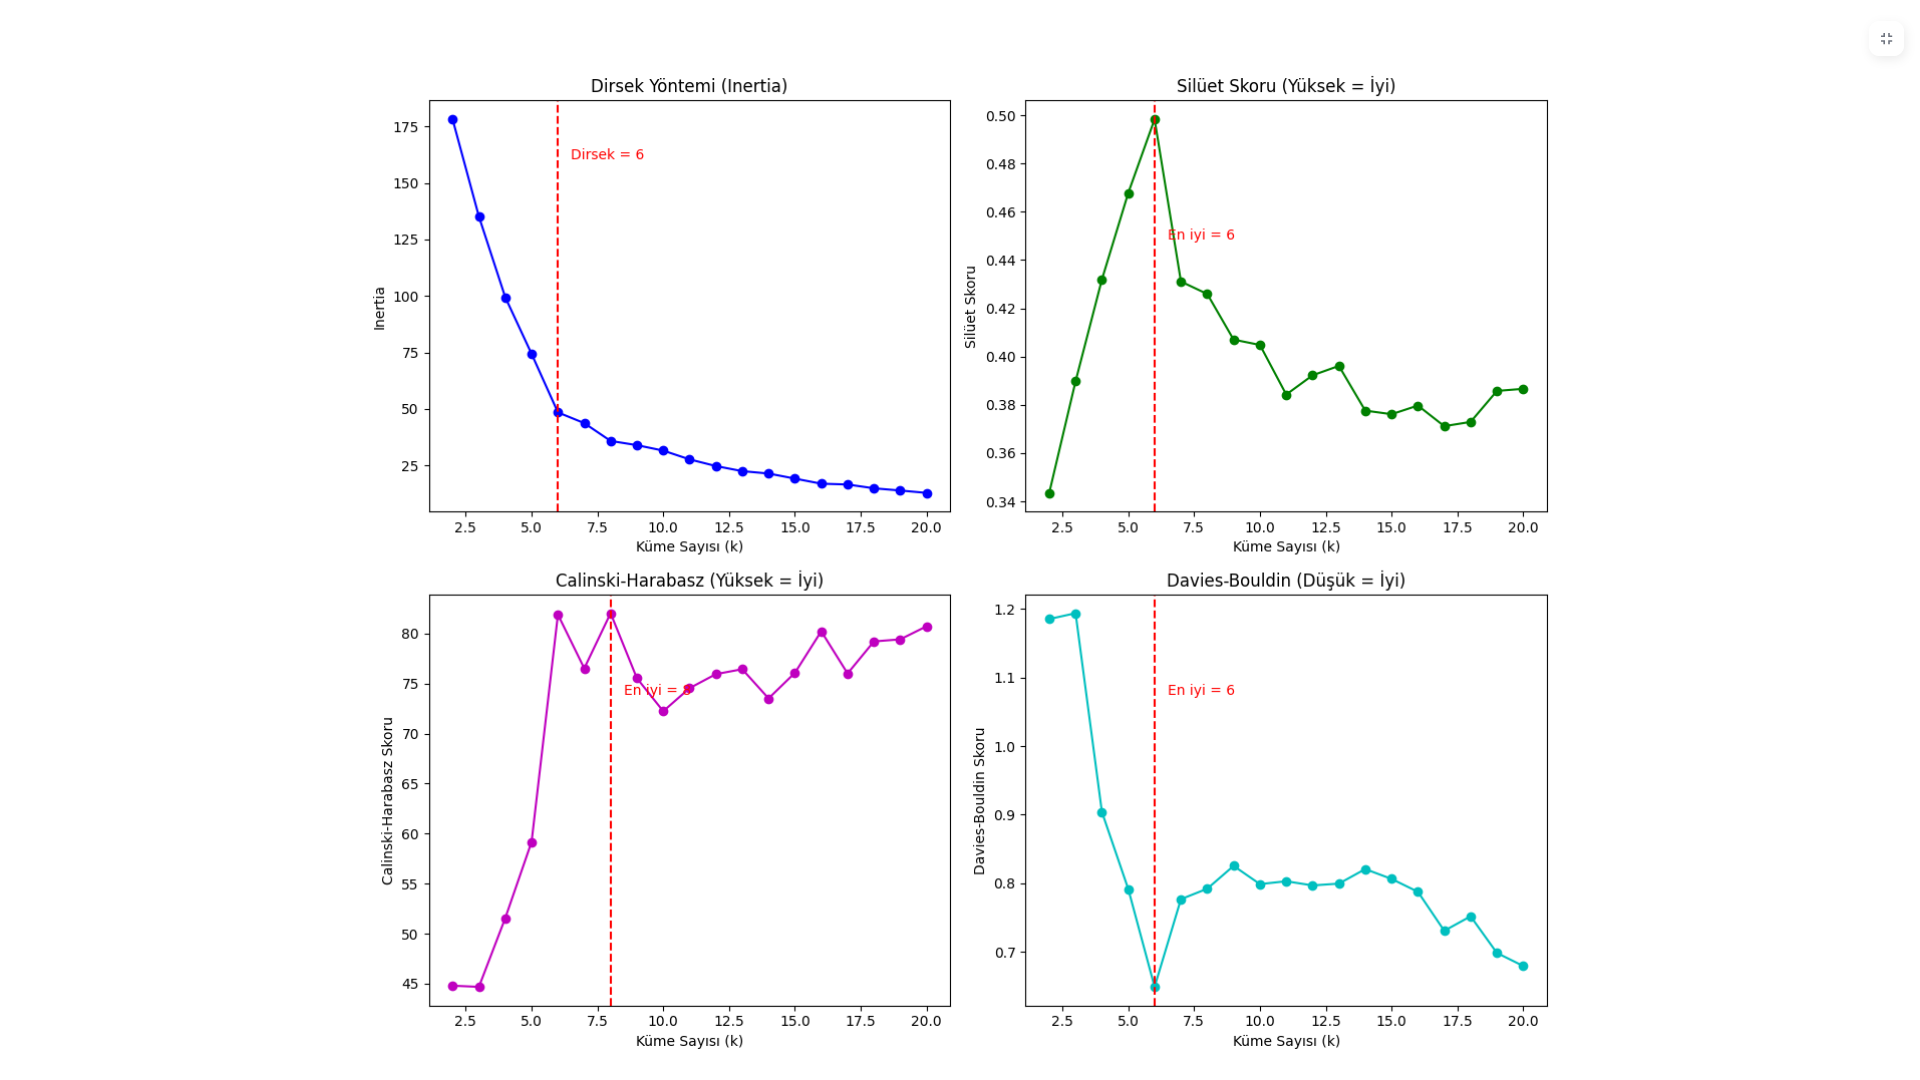
\includegraphics[width=0.8\textwidth]{images/optimal-kume-sayisi-analizi.png}
    \caption{Optimal Küme Sayısı Belirleme Analizi}
    \label{fig:optimal_clusters}
\end{figure}

Şekil \ref{fig:optimal_clusters}'de dirsek yöntemi ve silhouette analizi kullanılarak optimal küme sayısının belirlenmesi gösterilmektedir. Analiz, farklı K değerleri için WCSS (Küme İçi Kareler Toplamı) ve silhouette skoru metriklerini karşılaştırmaktadır.

\subsubsection{JSON Veri Yapısı ve İşleme}

Coraza WAF, günlük verilerini JSON biçiminde üretir \cite{coraza2023}. Sistem, iki farklı JSON yapısını destekler:

\textbf{1. İşlem Sarmalayıcı Biçimi:}
\begin{lstlisting}[language=json]
{
  "transaction": {
    "client_port": 12345,
    "request": {
      "uri": "/login",
      "method": "POST"
    },
    "timestamp": "2023-01-01T10:20:30Z",
    "is_interrupted": false
  }
}
\end{lstlisting}

\textbf{2. Düz Biçim:}
\begin{lstlisting}[language=json]
{
  "client_port": 12345,
  "request.uri": "/login", 
  "request.method": "POST",
  "timestamp": "2023-01-01T10:20:30Z",
  "is_interrupted": false
}
\end{lstlisting}

\newpage

\subsubsection{Analiz Stratejisi}

Sistem, uyarlanabilir analiz stratejisi kullanarak farklı veri kümeleri için en uygun analiz yaklaşımını belirler:

\textbf{Sıralı Analiz Aşamaları:}

\begin{enumerate}
    \item \textbf{Keşifsel Veri Analizi:} Veri dağılımı, bağıntı analizi
    \item \textbf{Özellik Seçimi:} Varyans eşiği, bağıntı filtreleme
    \item \textbf{SOM Eğitimi:} Izgara optimizasyonu, parametre ayarlama
    \item \textbf{Üst-Kümeleme:} Algoritma seçimi, doğrulama metrikleri
\end{enumerate}

\textbf{Duruma Özgü Analiz Seçimi:}

\begin{itemize}
    \item \textbf{Küçük Veri Kümeleri (n < 1000):} Doğrudan SOM eğitimi, basit görselleştirme
    \item \textbf{Orta Boyut Kümeler (1000 < n < 10000):} Toplu işleme, üst-kümeleme
    \item \textbf{Büyük Veri Kümeleri (n > 10000):} Artımlı öğrenme, dağıtık işleme
\end{itemize}

\textbf{Başarım Metriklerinin Seçim Ölçütleri:}

\begin{table}[!ht]
\centering
\caption{Analiz Metriklerinin Kullanım Alanları}
\label{tab:metrics_usage}
\begin{tabular}{|l|p{0.3\textwidth}|p{0.4\textwidth}|}
\hline
\textbf{Metrik} & \textbf{Kullanım Alanı} & \textbf{Avantajlar} \\
\hline
Silhouette Skoru & Küme kalitesi değerlendirme & Küme sıkılığı ve ayrılık ölçümü \\
\hline
Calinski-Harabasz & Optimal küme sayısı belirleme & Varyans oranı analizi \\
\hline
Davies-Bouldin & Küme kompaktlığı analizi & Düşük değerler iyi kümelemeyi gösterir \\
\hline
Niceleme Hatası & SOM temsil kalitesi & Eğitim yakınsama izleme \\
\hline
Topolojik Hata & Komşuluk korunması & Topoloji koruma değerlendirmesi \\
\hline
\end{tabular}
\end{table}

\newpage

\subsubsection{Calinski-Harabasz İndeksi}

\textbf{Calinski-Harabasz İndeksi Nedir?}

Calinski-Harabasz (CH) İndeksi, kümeleme kalitesini değerlendiren ve optimal küme sayısını bulmak için kullanılan bir metriktir. Bu indeks, kümeler arası ayrılık ile küme içi sıkılık oranını hesaplar.

CH İndeksinin çalışma prensibi:
\begin{enumerate}
    \item Kümeler arası varyans hesaplanır
    \item Küme içi varyans hesaplanır  
    \item Bu iki değerin oranı alınır ve serbestlik derecelerine göre düzeltilir
    \item Yüksek değer daha iyi kümelenme anlamına gelir
\end{enumerate}

CH İndeksinin avantajları:
- Optimal küme sayısını belirlemede etkili
- Hesaplama hızı yüksek
- Farklı küme şekilleri için genel olarak güvenilir
- Küme sayısı arttıkça nasıl değiştiğini takip etmek kolay

CH İndeksinin yorumlanması:
- \textbf{Yüksek değer:} İyi kümelenme, kümeler birbirinden ayrık ve içten sıkı
- \textbf{Düşük değer:} Zayıf kümelenme, kümeler belirsiz
- \textbf{Maksimum nokta:} Genellikle optimal küme sayısını gösterir

\textbf{Teknik Detaylar:}

\begin{equation}
CH = \frac{SS_B / (k-1)}{SS_W / (n-k)}
\label{eq:calinski_harabasz}
\end{equation}

Burada:
\begin{itemize}
    \item $SS_B$: Kümeler arası kareler toplamı
    \item $SS_W$: Küme içi kareler toplamı
    \item $k$: Küme sayısı
    \item $n$: Toplam veri noktası sayısı
\end{itemize}

\newpage

\subsubsection{Davies-Bouldin İndeksi}

\textbf{Davies-Bouldin İndeksi Nedir?}

Davies-Bouldin (DB) İndeksi, kümeleme kalitesini ölçen ve Calinski-Harabasz'ın tersine düşük değerlerin iyi olduğu bir metriktir. Her kümenin kendi içindeki dağılım ile en yakın komşu kümeye olan mesafesini karşılaştırır.

DB İndeksinin çalışma prensibi:
\begin{enumerate}
    \item Her küme için içindeki noktaların merkeze olan ortalama mesafesi hesaplanır
    \item Her küme için diğer küme merkezlerine olan mesafeler bulunur
    \item Her küme çifti için benzerlik oranı hesaplanır
    \item En kötü (en yüksek) benzerlik oranları toplanır ve ortalaması alınır
\end{enumerate}

DB İndeksinin avantajları:
- Küme kompaktlığını ve ayrılığını birlikte değerlendirir
- Hesaplama basit ve hızlı
- Küme şekillerinden görece bağımsız
- Optimal küme sayısını belirlemede kullanışlı

DB İndeksinin yorumlanması:
- \textbf{Düşük değer (0'a yakın):} Mükemmel kümelenme, kompakt ve ayrık kümeler
- \textbf{Yüksek değer:} Zayıf kümelenme, kümeler iç içe veya dağınık
- \textbf{Minimum nokta:} Optimal küme sayısını gösterir

\textbf{Teknik Detaylar:}

\begin{equation}
DB = \frac{1}{k} \sum_{i=1}^{k} \max_{j \neq i} \left( \frac{\sigma_i + \sigma_j}{d(c_i, c_j)} \right)
\label{eq:davies_bouldin}
\end{equation}

Burada:
\begin{itemize}
    \item $\sigma_i$: Küme $i$'nin içindeki noktaların merkeze olan ortalama mesafesi
    \item $d(c_i, c_j)$: Küme $i$ ve $j$ merkezleri arasındaki mesafe
    \item $k$: Küme sayısı
\end{itemize}

\newpage

\subsubsection{Topological Error}

\textbf{Topological Error Nedir?}

Topological Error (Topolojik Hata), SOM'un giriş verilerinin komşuluk ilişkilerini ne kadar iyi koruduğunu ölçen bir metriktir. SOM'un temel özelliklerinden biri olan "topology preservation" yeteneğini değerlendirir.

Topological Error'un çalışma prensibi:
\begin{enumerate}
    \item Her veri noktası için BMU (en yakın nöron) bulunur
    \item Aynı veri noktası için ikinci en yakın nöron belirlenir
    \item BMU ile ikinci en yakın nöronun SOM haritasında komşu olup olmadığı kontrol edilir
    \item Komşu değillerse, bu bir topolojik hata sayılır
    \item Tüm hatalar toplanır ve toplam veri sayısına bölünür
\end{enumerate}

Topological Error'un önemi:
- SOM'un topoloji koruma yeteneğini doğrular
- Düşük değer, SOM'un giriş uzayının yapısını iyi koruduğunu gösterir
- Grid boyutunun ve parametrelerin uygunluğunu değerlendirir
- Görselleştirme kalitesinin göstergesidir

Topological Error'un yorumlanması:
- \textbf{Düşük değer (0'a yakın):} Mükemmel topoloji korunması
- \textbf{Yüksek değer:} Topoloji bozulması, SOM parametreleri gözden geçirilmeli
- \textbf{0 değeri:} İdeal durum, tüm komşuluklar korunmuş

\textbf{Teknik Detaylar:}

\begin{equation}
TE = \frac{1}{N} \sum_{i=1}^{N} u(x_i)
\label{eq:topological_error}
\end{equation}

Burada:
\begin{equation}
u(x_i) = \begin{cases}
1 & \text{eğer BMU ve 2. BMU komşu değilse} \\
0 & \text{eğer BMU ve 2. BMU komşuysa}
\end{cases}
\label{eq:topological_error_function}
\end{equation}

\newpage

\subsection{Meta-Kümeleme Algoritmaları}

Sistem, SOM çıktısı üzerinde farklı kümeleme algoritmalarını uygular:

\subsubsection{K-Means Clustering}

\textbf{K-Means Algoritması Nedir?}

K-Means, veri setindeki noktaları önceden belirlenen sayıda (k) gruba ayıran bir kümeleme algoritmasıdır. Algoritmanın temel amacı, her bir veri noktasını en yakın küme merkezine atayarak, küme içi benzerliği maksimize etmek ve kümeler arası farklılığı artırmaktır.

Algoritma şu adımları takip eder:
\begin{enumerate}
    \item Küme sayısı (k) önceden belirlenir
    \item K adet merkez nokta rastgele yerleştirilir
    \item Her veri noktası, en yakın merkez noktaya atanır
    \item Her kümenin yeni merkez noktası, o kümedeki tüm noktaların ortalaması alınarak hesaplanır
    \item Merkez noktalar değişmeyene kadar 3. ve 4. adımlar tekrarlanır
\end{enumerate}

K-Means'in ana avantajı hesaplama hızı ve basitliğidir. Ancak küme sayısının önceden bilinmesi gerekir ve küresel olmayan küme şekillerinde başarısız olabilir.

\textbf{Teknik Detaylar:}

\begin{equation}
J = \sum_{i=1}^{k} \sum_{x \in C_i} ||x - \mu_i||^2
\label{eq:kmeans_objective}
\end{equation}

Burada $\mu_i$ küme merkezleridir.

\newpage

\subsubsection{DBSCAN Algorithm}

\textbf{DBSCAN Algoritması Nedir?}

DBSCAN (Density-Based Spatial Clustering of Applications with Noise), veri yoğunluğuna dayalı olarak kümeleme yapan bir algoritmadır. K-Means'ten farklı olarak, küme sayısını önceden belirleme gerektirmez ve keyfi şekillerdeki kümeleri tespit edebilir.

Algoritmanın temel prensibi, belirli bir yarıçap içerisinde yeterli sayıda komşuya sahip noktaları "yoğun bölgeler" olarak tanımlamak ve bu bölgeleri genişleterek kümeleri oluşturmaktır. Yeterli komşuya sahip olmayan noktalar ise gürültü (noise) olarak sınıflandırılır.

DBSCAN'in çalışma mantığı:
\begin{enumerate}
    \item Her veri noktası için epsilon ($\varepsilon$) yarıçapındaki komşu sayısı hesaplanır
    \item Eğer bir nokta minimum nokta sayısından (MinPts) fazla komşuya sahipse "çekirdek nokta" olur
    \item Çekirdek noktalardan başlayarak, komşu noktalar aynı kümeye dahil edilir
    \item Bu işlem tüm erişilebilir noktalar kümeye dahil edilene kadar devam eder
    \item Hiçbir kümeye dahil olmayan noktalar gürültü olarak işaretlenir
\end{enumerate}

DBSCAN'in ana avantajları:
- Küme sayısını önceden belirleme gerektirmez
- Keyfi şekillerdeki kümeleri bulabilir
- Gürültü noktalarını otomatik tespit eder
- Farklı yoğunluktaki kümeleri işleyebilir

\textbf{Teknik Detaylar:}

DBSCAN (Density-Based Spatial Clustering of Applications with Noise), yoğunluk tabanlı kümeleme algoritmasıdır. İki temel parametre kullanır: $\epsilon$ (komşuluk yarıçapı) ve $MinPts$ (minimum nokta sayısı).

\newpage

\textbf{Temel Tanımlar:}

\textbf{1. $\epsilon$-Neighborhood (Epsilon Komşuluğu):}
Bir nokta $p$'nin $\epsilon$-komşuluğu aşağıdaki şekilde tanımlanır:

\begin{equation}
N_{\epsilon}(p) = \{q \in D | \text{dist}(p,q) \leq \epsilon\}
\label{eq:epsilon_neighborhood}
\end{equation}

\textbf{2. Core Point (Çekirdek Nokta):}
Bir nokta $p$, eğer $|N_{\epsilon}(p)| \geq MinPts$ koşulunu sağlıyorsa core point'tir.

\begin{equation}
\text{CorePoint}(p) = |N_{\epsilon}(p)| \geq MinPts
\label{eq:core_point}
\end{equation}

\textbf{3. Border Point (Sınır Nokta):}
Bir nokta $p$, core point değilse ancak en az bir core point'in $\epsilon$-komşuluğunda yer alıyorsa border point'tir.

\textbf{4. Noise Point (Gürültü Nokta):}
Ne core point ne de border point olan noktalar noise point olarak sınıflandırılır.

\textbf{Yoğunluk Bağlantısı (Density Connectivity):}

\textbf{Directly Density-Reachable:}
Nokta $q$, nokta $p$'den directly density-reachable'dır eğer:
\begin{itemize}
    \item $q \in N_{\epsilon}(p)$ ve
    \item $p$ bir core point ise
\end{itemize}

\textbf{Density-Reachable:}
Nokta $q$, nokta $p$'den density-reachable'dır eğer $p_1, p_2, ..., p_n$ nokta zinciri mevcutsa:
$p_1 = p$, $p_n = q$ ve her $p_{i+1}$ nokta $p_i$'den directly density-reachable'dır.

\textbf{Density-Connected:}
İki nokta $p$ ve $q$ density-connected'dır eğer bir $o$ noktası mevcutsa hem $p$ hem de $q$ bu noktadan density-reachable'dır.

\newpage

\textbf{DBSCAN Parametre Seçimi:}

\begin{itemize}
    \item \textbf{$\epsilon$ Belirleme:} K-distance grafik metoduyla optimal $\epsilon$ değeri bulunur
    \item \textbf{MinPts Seçimi:} Genellikle $MinPts = 2 \times \text{boyut}$ kuralı kullanılır
    \item \textbf{Sistemde Kullanılan Değerler:} $\epsilon = 0.5$, $MinPts = 5$
\end{itemize}

\textbf{DBSCAN Avantajları:}
\begin{itemize}
    \item Küme sayısını önceden belirleme gerektirmez
    \item Gürültü noktalarını otomatik tespit eder
    \item Keyfi şekilli kümeleri bulabilir
    \item Outlier detection capability'si
\end{itemize}

\subsubsection{Hierarchical Clustering}

\textbf{Hiyerarşik Kümeleme Nedir?}

Hiyerarşik kümeleme, veri noktaları arasındaki mesafe ilişkilerini kullanarak ağaç benzeri (dendrogram) bir küme yapısı oluşturan algoritmadır. Bu algoritma, farklı küme sayıları için sonuçları aynı anda görebilme avantajı sağlar.

İki ana türü vardır:

\textbf{1. Aglomeratif (Agglomerative) Kümeleme:}
- Alt-yukarı (bottom-up) yaklaşım kullanır
- Her veri noktası kendi kümesi olarak başlar
- En yakın kümeleri tekrar tekrar birleştirerek büyük kümeler oluşturur
- Tüm noktalar tek kümede toplanana kadar devam eder

\textbf{2. Bölen (Divisive) Kümeleme:}
- Yukarı-alt (top-down) yaklaşım kullanır
- Tüm veriler tek kümede başlar
- En uzak alt grupları ayırarak küçük kümeler oluşturur
- Her nokta kendi kümesinde kalana kadar devam eder

Hiyerarşik kümelemenin ana avantajları:
- Dendrogram ile küme yapısının görselleştirilmesi
- Farklı küme sayıları için sonuçların eş zamanlı elde edilmesi
- Deterministik sonuçlar (rastgelelik yok)
- Küme sayısını önceden belirleme gerektirmez

\newpage

Ana dezavantajı, büyük veri setlerinde yüksek hesaplama maliyetidir (O(n³)).

\textbf{Teknik Detaylar:}

Linkage criteria için üç farklı yöntem desteklenir:

\begin{itemize}
    \item \textbf{Single Linkage:} $d(C_i, C_j) = \min_{x \in C_i, y \in C_j} d(x,y)$
    \item \textbf{Complete Linkage:} $d(C_i, C_j) = \max_{x \in C_i, y \in C_j} d(x,y)$
    \item \textbf{Average Linkage:} $d(C_i, C_j) = \frac{1}{|C_i||C_j|} \sum_{x \in C_i} \sum_{y \in C_j} d(x,y)$
\end{itemize}

\subsection{Boyut İndirgeme Teknikleri}

\subsubsection{Principal Component Analysis (PCA)}

PCA, varyansı maksimize eden linear transformation kullanır:

\begin{equation}
Y = XW
\label{eq:pca_transform}
\end{equation}

Burada $W$ eigenvector matrix'idir.

\subsubsection{t-SNE (t-Distributed Stochastic Neighbor Embedding)}

t-SNE, yüksek boyutlu benzerlik dağılımını düşük boyutta korur:

\begin{equation}
C = \sum_i \sum_j p_{ij} \log \frac{p_{ij}}{q_{ij}}
\label{eq:tsne_cost}
\end{equation}

\newpage

\subsubsection{UMAP (Uniform Manifold Approximation and Projection)}

UMAP, manifold structure'ı koruyarak boyut indirgeme yapar:

\begin{table}[!ht]
\centering
\caption{Boyut İndirgeme Tekniklerinin Karşılaştırması}
\label{tab:dim_reduction_comparison}
\begin{tabular}{|l|c|c|c|c|}
\hline
\textbf{Teknik} & \textbf{Lineer} & \textbf{Hız} & \textbf{Global Yapı} & \textbf{Local Yapı} \\
\hline
PCA & Evet & Çok Hızlı & İyi & Zayıf \\
\hline
t-SNE & Hayır & Yavaş & Zayıf & Mükemmel \\
\hline
UMAP & Hayır & Hızlı & İyi & İyi \\
\hline
\end{tabular}
\end{table}

\subsection{Sistem Mimarisi Detayları}

\subsubsection{Flask API Servisleri}

Sistem, mikroservis mimarisi ile iki farklı Flask API servisi kullanır:

\textbf{Flask Log API (Port 5000):}

Jenkins pipeline içerisinde dinamik olarak oluşturulan Flask uygulaması:

\begin{lstlisting}[language=python]
from flask import Flask, jsonify
import json, os

app = Flask(__name__)
LOG_PATH = "./coraza/reports/audit.log"

@app.route('/logs', methods=['GET'])
def get_logs():
    logs = []
    with open(LOG_PATH, 'r') as f:
        for line in f:
            try:
                logs.append(json.loads(line.strip()))
            except json.JSONDecodeError:
                continue
    return jsonify(logs)

if __name__ == '__main__':
    app.run(host='0.0.0.0', port=5000)
\end{lstlisting}

\newpage

\subsubsection{Veri Akışı ve Sistem Entegrasyonu}

Sistem veri akışı şu şekilde çalışır:

\begin{enumerate}
    \item \textbf{Boru Hattı Başlatma:} CorazaWAF-Log-Last boru hattı başlatılır
    \item \textbf{Ortam Kurulumu:} Go, Flask kurulumu ve bağımlılık yönetimi
    \item \textbf{WAF Derleme:} Coraza WAF v3 ikili dosya derleme
    \item \textbf{Servis Başlatma:} WAF port 8091, Flask API port 5000'de başlatılır
    \item \textbf{Güvenlik Tarama:} ZAP tarayıcısı hedef URL'yi tarar
    \item \textbf{Log Üretimi:} WAF JSON \texttt{audit.log} üretir
    \item \textbf{Veri Analizi:} Streamlit modülü API'den veri alır ve işler
\end{enumerate}

\subsection{Validasyon ve Güvenilirlik Stratejileri}

\subsubsection{Çapraz Doğrulama Metodolojisi}

\begin{itemize}
    \item \textbf{K-Katlı Çapraz Doğrulama:} SOM parametre optimizasyonu
    \item \textbf{Bootstrap Örnekleme:} Güven aralıkları hesaplama  
    \item \textbf{Permütasyon Testi:} İstatistiksel anlamlılık testi
    \item \textbf{Kararlılık Analizi:} Kümeleme tutarlılığı değerlendirmesi
\end{itemize}

\subsubsection{Performans İzleme}

Sistem performansı sürekli izlenir:

\begin{itemize}
    \item \textbf{Bellek Kullanımı:} Gerçek zamanlı RAM izleme
    \item \textbf{İşleme Süresi:} Algoritma yürütme takibi
    \item \textbf{Doğruluk Metrikleri:} Kümeleme kalitesi değerlendirmesi
    \item \textbf{Hata Oranları:} Sistem arıza tespiti
\end{itemize}

Bu kapsamlı metodoloji, sistemin güvenilir ve ölçeklenebilir bir şekilde çalışmasını sağlamaktadır.











